

%%%%%%%%%%%%%%%%%%%%%%%%%%%%
% SECTION                  %
%%%%%%%%%%%%%%%%%%%%%%%%%%%%
%\addcontentsline{toc}{chapter}{Chapitre 1 : Introduction générale} 
\section{Introduction}
\label{chap:sectionone}
Avant l'implémentation d'une solution informatique, il est primordial de réaliser une étude et de préparer le contexte du projet. Donc, le chapitre initial se focalisera sur la présentation de l'organisme d'accueil, le contexte et le cadre professionnel du projet. Par la suite, nous procédons à une description et à une critique des solutions existantes tout en expliquant la gestion d'une entreprise, en respectant Les définitions des termes techniques utilisés. Finalement, nous présentons la solution 
proposée et ses buts, ainsi que la méthode de travail utilisée.




\section{Présentation de l'organisme d'acceuil}
Inno Think IT est une entreprise renommée de développement informatique est un fournisseur leader des solutions logicielles, basée en Tunisie et établie en 2015.
 Ils sont spécialisés dans une large gamme de services incluant le développement d'applications mobiles et web, l'analytique avancée et les solutions cloud. Leur équipe conçoit avec expertise des logiciels sur mesure, des applications de bureau aux plateformes SaaS avancées, assurant une efficacité opérationnelle et un engagement numérique supérieur. Chez InnoThink, ils lient entre la technologie et la créativité pour stimuler la croissance des entreprises et livrer des projets de haute qualité dans les délais.

 \begin{figure}[h]%
    \center%
    
\includegraphics[width=0.5\textwidth]{pages/images/innothink.png}
    \caption{Logo de l'entreprise }
    \label{fig:test}%
  \end{figure}

\subsection{Les activités de InnoThink}
De plus de 7 ans, InnoThink propose des réponses globales aux moyennes et  aux grandes entreprises, organisation privée ou publique, quel que soit leur secteur d'activité, leur complexité organisationnelle ou leur localisation.
\\
En effet, Innothink s'occupe de certains services tels que;
\begin{itemize}

    \item Dévelopement web
    \item Développement d'application
    \item Développement E-commerce
    \item Dévelopement Blockchain
    \item Dévelopement jeux
    \item Solutions salesforce
    \item IA/ ML 
    \item IOT et systémes embarqués
    \item  DevOPs
\end{itemize}
\subsection{InnoThink Academy}
InnoThink propose des programmes de formation spécialisés conçus pour renforcer l'efficacité et l'adaptabilité de ses équipe dans le marché rapide d'aujourd'hui. ses cours sont structurés pour fournir non seulement des connaissances théoriques mais aussi des compétences pratiques immédiatement applicables dans votre cadre professionnel.
Elle offre une gamme complète de cours de développement, disponibles à la fois en salle de classe et en ligne, conçus pour améliorer les compétences professionnelles dans diverses industries.

\section{Présentation du projet}
Avant de commencer tout projet, une compréhension détaillée de la situation actuelle est 
cruciale.\\
InnoThink possède une large communité de collaborateurs qui ont besoin
d'améliorer leurs compétences synchronisant aux demandes des clients au sein de la société afin d'obtenir les projets complets dans la date précise et cela prend du temps pour former les collaborateurs individuellement ce qui met en risque le finissement du travail.

\vspace{5mm}
\subsection{Problématique}

InnoThink doit gérer la réalisation des projets des diverses techniques et complexité  dans un court temps. Malheureusement, il y a des collaborateurs qui manquent de connaissances pour les nouveaux techniques inventés. Cette situation génère un certain obstacle pour la réalisation des projets au délai précis.



\section{Etude de l'existant}
\subsection{Analyse de l'existant}
Notre projet nous a permis de faire une recherche sur les applications d’E-learning
Existant sur le marché tel que : FreeCode Camp et HakerRank
Ce sont deux plateformes d’E-learning en ligne qui offrent plusieurs fonctionnalités
dont on a besoin pour note application telle que les quiz, Certificats et un espace
d’interaction, etc.

\newpage
\textbf{FreeCodeCamp } a a été lancé en octobre 2014 et incorporé sous le nom de Free Code Camp, Inc. Le fondateur, Quincy Larson, est un développeur de logiciels
Les ressources sont des cours textes sur le développement informatique ou bien sous format vidéo. Chaque cours possède des quiz à la fin de chaque section. À la fin de chaque tutoriel on peut avoir un certificat de réussite après avoir obtenu un minimum de seuils sur les quiz et les mini-projets.
\begin{figure}[ht]%
    \center%
    
\includegraphics[width=0.6\textwidth]{pages/images/freecodecamp.png}
    \caption[Figure 1:]{Présentation du plateforme FreeCodeCamp}\label{fig:test}%
  \end{figure}
  \\
  La plateforme donne accès aux différents chapitres de la formation et on peut le visualiser facilement comme le montre la figure suivante
  \\
\begin{figure}[ht]%
    \center%
    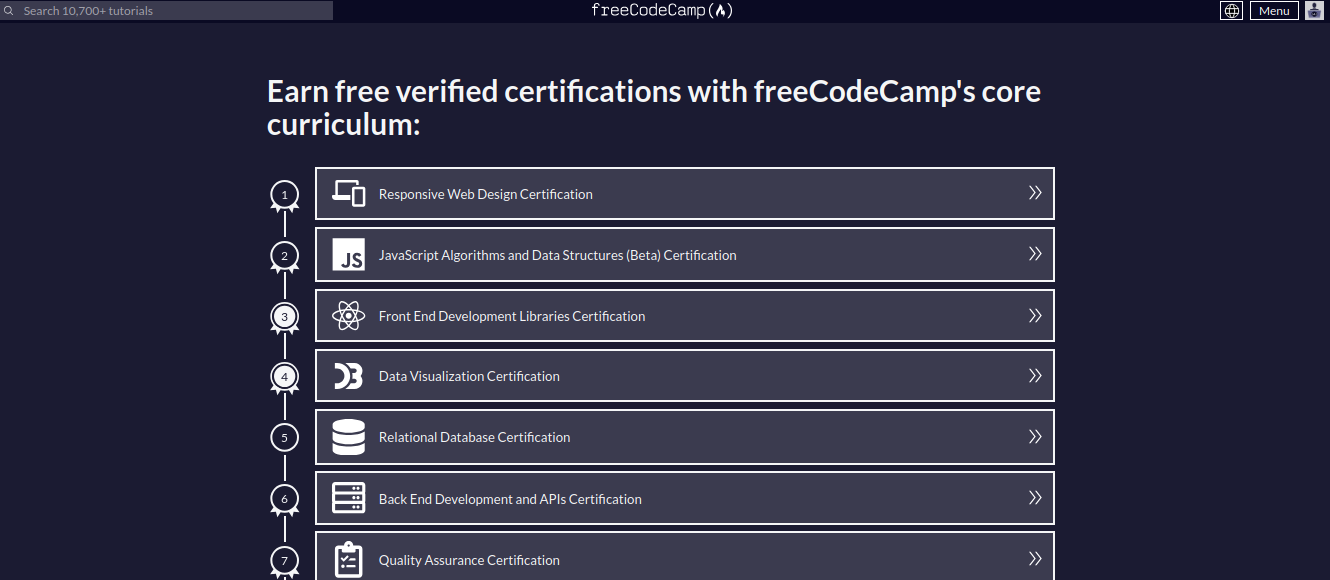
\includegraphics[width=0.6\textwidth]{pages/images/freecodecamp2.png}
    \caption[Figure 1:]{Présentation des cours du plateforme FreeCodeCamp}\label{fig:test}%
  \end{figure}
  \newline
\textbf{HackerRank}
 est une entreprise spécialisée dans les concours de programmation pour développeurs et entreprises.
 \\Les concours de programmation d'HackerRank utilisent une multitude de langages (Java, C++, PHP, SQL, etc. ) et couvrent de nombreux domaines de l'informatique.

\begin{figure}[ht]%
    \center%
    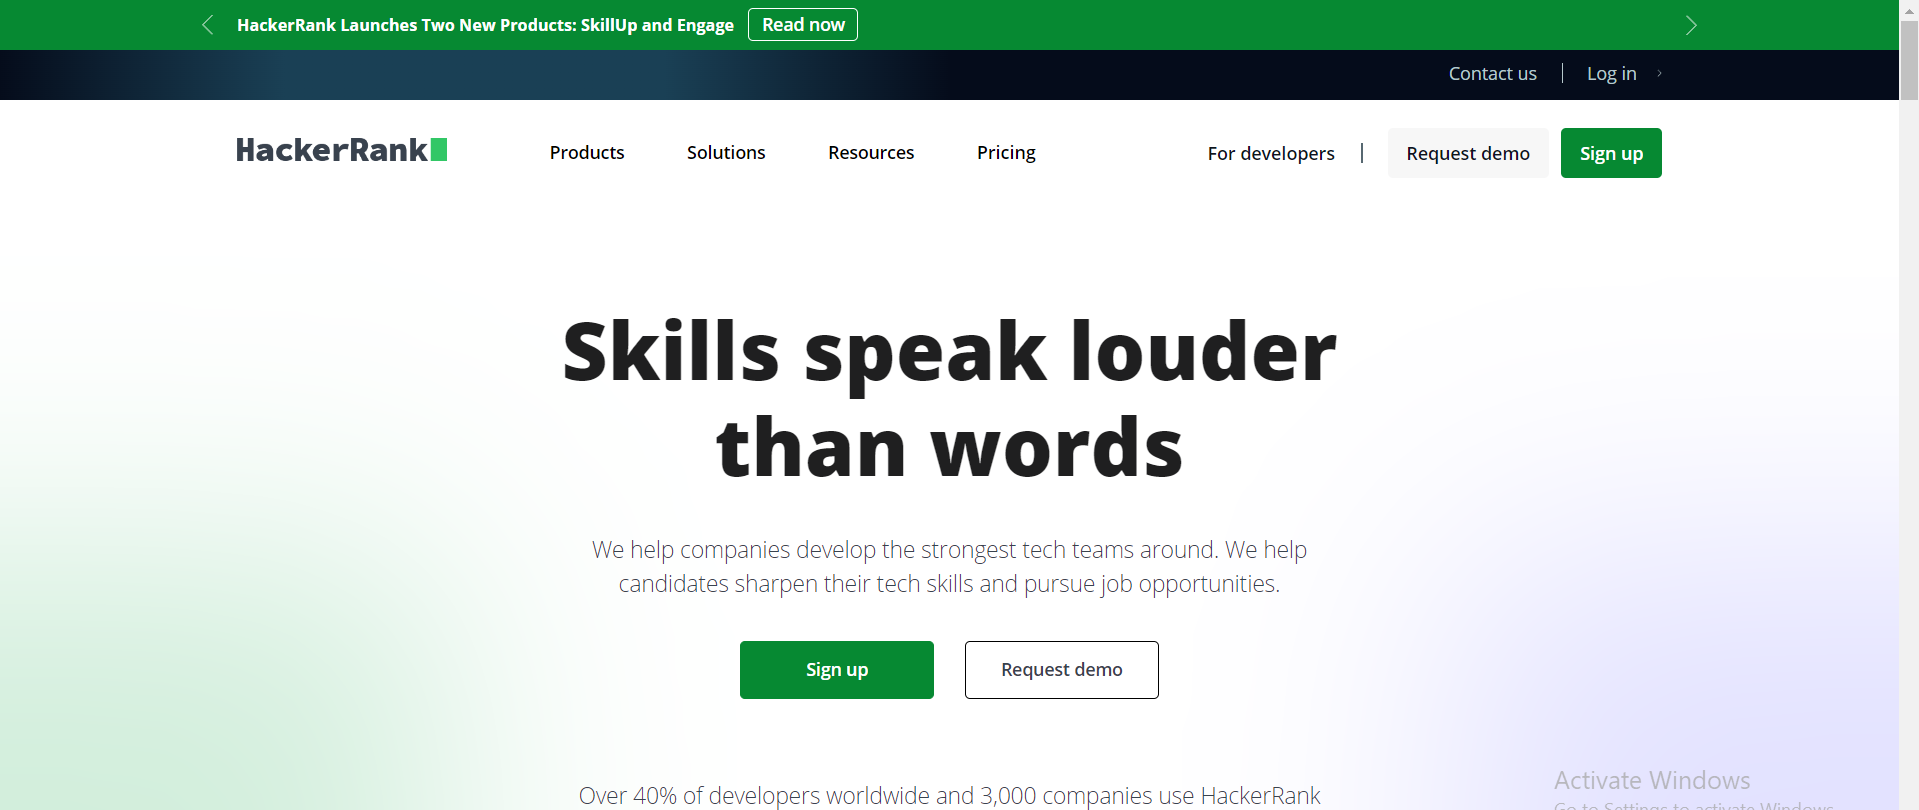
\includegraphics[width=0.6\textwidth]{pages/images/hackeRrank.png}
    \caption{Présentation du plateforme HackerRank}\label{fig:test}%
  \end{figure}
\subsection{Critique de l'existant}
FreeCodeCamp et HackerRank sont deux plateformes d'E-learning. On a eu
l’opportunité d’y accéder en tant que tuteur et étudiant afin de découvrir ses différends
fonctionnalités.
\\
Plusieurs insuffisances ont été détectées à savoir ;
\begin{itemize}
    
\item  Une défaillance de l’ergonomie
\item L’absence du du controle simultané, on y trouve plutôt des exercies standards 
\item  Pas d’espace réservé pour les exercices demandés ou les apprenants peuvent échanger des exercices entre eux et pas d’indexation sur les exercices présents sur la plateforme.
\item Absence d’une matrice des experts selon leurs compétences qui permet à l’apprenant
de consulter leurs coordonnées.

\begin{figure}[ht]%
    \center%
    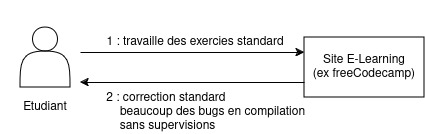
\includegraphics[width=0.8\textwidth]{pages/images/porblem.jpg}
    \vspace{3mm}
    \caption{Présentation du problématique}\label{fig:test}%
  \end{figure}

\vspace{10mm}
\subsection{Solutions proposé}
La solution que nous proposons consiste à concevoir et développer une plateforme
baptisée au sein InnoThink Académie nommée CodeNest . Cette application offre plusieurs volets comme l’E-Learning, Blended Learning, Social Learning et mobile Learning.
\begin{itemize}
    \item Knowledge-Base : C’est une base de documents confidentiels de InnoThink
consultables non téléchargeables.
\item Expert-Base : C’est une base des experts qui vont générer une liste de support de cours contenant des exercices 
\end{itemize}
Par ailleurs CodeNest  est une plateforme de partage de
connaissances entre les différents collaborateurs et sert aussi de référentiel pour le suivi des
parcours de compétences et de carrières pour les collaborateurs.
\vspace{5mm}
\begin{figure}[ht]%
    \center%
    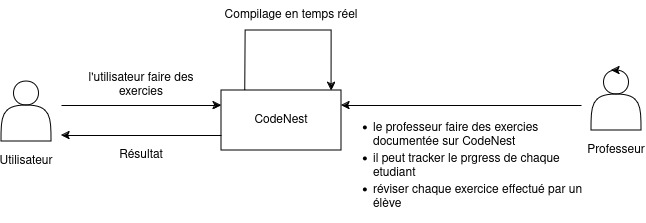
\includegraphics[width=1\textwidth]{pages/images/asma-solution.jpg}
    \vspace{3mm}
    \caption{Présentation de la solution proposée}\label{fig:test}%
  \end{figure}

\section{Méthodologie de travail et formalisme des modelisations}
Dans cette partie, nous allons définir la méthode de travail ainsi que le choix d'utilisation
\subsection{Language de modelisation}
L'UML (Unified Modeling Language) est la  Langage de modélisation unifié, et un langage de modélisation graphique est une méthode normalisée qui permet de présenter les besoins du projet sous forme de diagramme .
\\À noter que l'UML n'est pas une méthode mais une démarche qui se base sur une approche objet:
\\UML possède 3 principes fondamentaux :
\begin{itemize}
\item Guidée par les besoins du client;
\item Basé sur le diagramme de classes où on trouve les différentes entités avec les
attributs et les différentes fonctionnalités et les autres diagrammes nous permettent
d’avoir une vue détaillée sur les besoins
\item démarche itératif et incrémental
\end{itemize}
% \vspace{10mm}
\subsection{Méthodologie de travail}
{\bf{Méthode agile:}}
Le plateforme que nous souhaitons développer est à la fois dynamique et complexe, et que notre domaine d'activité est l'éducation ainsi que  la méthodologie la plus conseillée est le Scrum.
L'interaction entre l'équipe de développement, les consultants et le client est un aspect crucial dans la méthodologie agile.

\vspace{8mm}

{\bf{ Scrum :}}est un framework ou cadre de développement complexe qui est conçu pour aider les équipes à travailler ensemble de manière plus efficace et productive.

La figure représente les principales étapes de la méthodologie Scrum, chacune d'entre eux implique de différents processus à suivre.
\begin{figure}[H]%
    \center%
    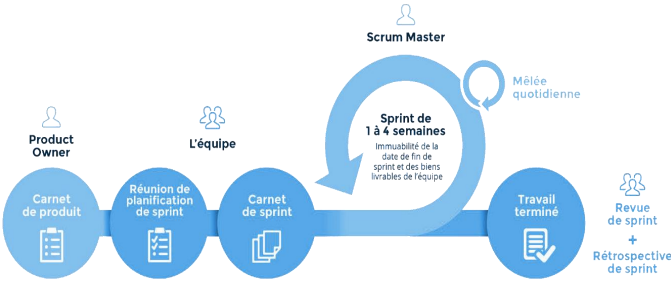
\includegraphics[width=0.6\textwidth]{pages/images/scrum.png}
    \caption{La méthodologie Scrum}\label{fig:test}%
  \end{figure}

\vspace{8mm}

 {\bf{ Sprint :}}La planification du sprint comprend l’identification des points prioritaires que l’équipe pense pouvoir réaliser au cours du sprint.

La revue du sprint a lieu à la fin de chaque sprint où l’équipe de développement présente les fonctionnalités terminées. L’incrément produit est éventuellement livrable et la mise en place du prochain sprint peut être anticipée.



  
\subsection{Choix de la méthode}
Nous avons choisi d’utiliser la méthode de SCRUM afin de gérer notre projet. Cette
méthode va nous permettre, en cas de besoin, d’ajouter ou de modifier des fonctionnalités au
niveau d’un sprint désiré sans affecter les autres. En plus, cette méthode nous permettra
de mieux respecter les dates planifiées pour clôturer les différents sprints.






 


\section{Conclusion}
Ce chapitre commence par la présentation du cadre global de notre projet,
en exposant l’organisation qui nous accueille, c’est la solution que nous proposons afin de minimiser la durée de formation en Innothink.
\\Dans le chapitre suivant, nous allons représenter les
différents besoins susmentionnés sous forme de diagrammes UML (Unified
Modeling Language) et de sprints.

